%!TEX root = ./main.tex
\section{Inner Product Spaces}
\subsubsection*{Motivation}
\begin{definition}
    In $\b R^n$, the dot product of $\vec x$ and $\vec y$ is defined by  
\[ \vec x \cdot \vec y := x_1y_1 + x_2y_2 + \cdots + x_ny_n\]
for $\vec x = (\li xn), \vec y = (\li yn)$.
\end{definition}
\subsection{Inner Product and Norms}
\subsubsection*{Settings}
$V$ is a vector space over $\b F$, we can define the following mapping $ \la \ast, \ast \ra : V \times V \to \b F$.
\begin{definition}
$\la \cdot, \cdot \ra$ is called an inner product if it satisfying the following rules:
\begin{enumerate}
    \item(additivity in the first slot) $\la \vec v + \vec u, \vec w \ra = \la \vec v + \vec w \ra + \la \vec u, \vec w \ra, \ \forall \vec v, \vec u, \vec w \in V$
    \item(homogeneity in the first slot) $\la \lambda \vec v, \vec w \ra = \lambda \la \vec v + \vec w \ra, \ \forall \vec v \vec u, \vec w \in V, \lambda \in \b F$
    \item(conjugate symmetry) $\la \vec v, \vec w \ra = \overline{\la \vec w, \vec v \ra}, \ \forall \vec v,\vec w \in V$
    \item(positivity) $\la \vec v, \vec v \ra \geq 0, \ \forall \vec v \in V$
    \item(definiteness) $\la \vec v, \vec v \ra = 0$ iff $\vec v = \vec 0$.
\end{enumerate}
\end{definition}
\begin{question}
What about linearity in the second slot?
\end{question}
\begin{answer} We can compute
\[ \la \vec v, \vec u + \vec w \ra = \overline{\la \vec u + \vec w, \vec v\ra} = \overline{\la \vec u, \vec v \ra + \la \vec w, \vec v \ra} = \overline{\la \vec u, \vec v \ra} + \overline{\la \vec w, \vec v\ra } = \la \vec v, \vec u\ra + \la \vec v, \vec w\ra\]
\[ \la \vec v, \lambda \vec u\ra = \overline{\la \lambda \vec u, \vec v\ra} = \overline{\lambda \la \vec u,\vec v\ra} = \bar \lambda \ \overline{\la \vec u, \vec v\ra} = \bar \lambda \la \vec v, \vec u \ra\]
Not quite. \frownie{}
\end{answer}
\begin{remark}
    If $\vec v \in V$ is fixed then the function $\la \ast, \vec v \ra : \vec u \mapsto \la \vec u, \vec v \ra$ is a function functional. 
\end{remark}
\begin{example}
    On $\b R^n$, we could use any function of the type
    \[ c_1x_1y_1 + c_2x_2y_2 + \cdots + c_nx_ny_n\] where all $c_j \in \b R^+$.
\end{example}
\begin{remark}[Generalization to $\b C^n$]
    The inner product of this form of the standard product to $\b C^n$ can be defined as
    \[ \la \vec x, \vec y \ra = x_1\bar y_1 + x_2\bar y_2 + \cdots + x_n\bar y_n\]
\end{remark}
\begin{remark}[Generalization to any function space]
    \[ \la f, g \ra : = \int_D f(t)\overline{g(t)} dt\]
    or generally \[ \la f, g \ra : = \int_D f(t)\overline{g(t)}w(t) dt\]
    where $w(t)$ is the positive weight function. e.g. if $V = \c P(\b R)$, or $V = \c P(\b C)$, then 
    \[ \la f, g \ra : = \int_0^\infty f(t)\overline{g(t)}e^{-t} dt\]
\end{remark}
\begin{definition}
    For $\vec v \in V$, the (Euclidean) Norm is defined as
    \[ ||\vec v|| : = \sqrt{\la \vec v,\vec v \ra}\] 
\end{definition}
\begin{theorem}(Properties of Norms)
    \begin{enumerate}
        \item $||\lambda \vec v || = |\lambda| \ ||\vec v|| \ \forall \vec v \in V, \forall \lambda \in \b F $
        \item $||\vec v|| > 0$ for all $\vec v \in V$
        \item $||\vec v|| = 0$ if and only if $\vec v = \vec 0$ 
    \end{enumerate}
\end{theorem}
\begin{definition}
    An inner product space is a vector space $V$ along with and inner product on $V$.
\end{definition}
\begin{definition}
    For $\vec u,\vec v \in V$, we say $\vec u$ and $\vec v$ is orthogonal if $\la \vec u, \vec v\ra = 0$
\end{definition}
\begin{theorem}[Pythagorean Theorem] $ $
\begin{center}
    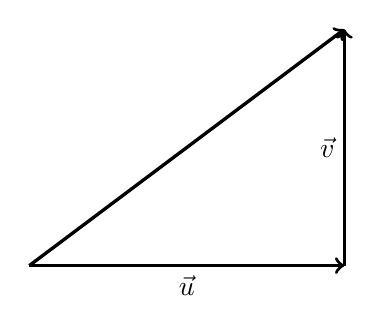
\begin{tikzpicture}
        \draw[->, very thick] (4,0) -- (4,3);
        \draw[->, very thick] (0,0) -- (4,0);
        \draw[->, very thick] (0,0) -- (4,3);
        \draw (2,0) node[anchor = north] {$\vec u$};
        \draw (4,1.5) node[anchor = east] {$\vec v$};
    \end{tikzpicture}
\end{center}
\[ ||\vec u + \vec v||^2 = ||\vec u||^2 + ||\vec v||^2 \iff \la \vec u + \vec v, \vec u + \vec v\ra = \la \vec u, \vec u \ra + \la \vec v, \vec v \ra \]
\end{theorem}
\begin{proof} We compute
    \[ \la \vec u + \vec v, \vec u + \vec v\ra = \la \vec u,\vec u \ra + \la \vec u , \vec v \ra + \la \vec v, \vec u \ra + \la \vec v,\vec v \ra = \la \vec u,\vec u \ra + 0 + 0 + \la \vec v,\vec v \ra = ||\vec u|| + ||\vec v|| \]
\end{proof}
\subsubsection*{Obeservation}
Given $\vec u,\vec v \in V$ such that $\vec v \neq 0$, we want to modify $\vec u$ such that $\vec u + c\vec v$ is orthogonal to $\vec v$. We know that $\la \vec v + c\vec v, \vec v \ra = 0$, solve for $c$ gives $c = \displaystyle\frac{-\la \vec u, \vec v\ra}{\la \vec v, \vec v \ra}$.
\begin{center}
    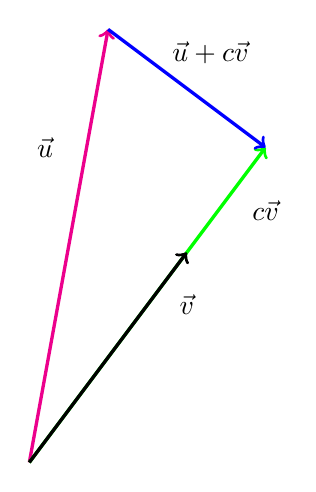
\begin{tikzpicture}
        \draw[->, very thick, color = magenta] (0,0) -- (1, 5.5);
        \draw[->, very thick, color = green] (0,0) -- (3, 4);
        \draw[->, very thick] (0,0) -- (2,2.66666666);
        \draw[->, very thick, color = blue] (1, 5.5) -- (3,4);
        \draw (2,2) node {$\vec v$};
        \draw (0.2,4) node {$\vec u$};
        \draw (3,3.2) node {$c\vec v$};
        \draw (2.3, 5.2) node {$\vec u + c\vec v$};
    \end{tikzpicture} 

    An orthogonal decompostion
\end{center}
\begin{theorem}[Cauchy-Schwarz Inequality]
    For any $u,v \in V$ where $V$ is a inner product space, the following holds
    \[ |\la \vec u,\vec v \ra| \leq ||\vec u|| \cdot ||\vec v||\]
\end{theorem}
\begin{proof}
    Given $\vec u,\vec v \in V$, we can assume without the loss of generality that $\vec v \neq 0$. So we can consider vectors $\vec u + c\vec v$ and $\vec v$ that are orthogonal for the choice that 
    \[ c: = \frac{ - \la \vec u,\vec v \ra}{\la \vec v,\vec v\ra}\]
    By Pathgrathrean theorem, $||\vec u + c\vec v||^2 + ||c\vec v||^2 = ||\vec u||^2$. But $||c\vec v||^2 = |c|^2||\vec v||^2$ and recall \[ c= \frac{- \la \vec u,\vec v\ra}{\la \vec v,\vec v\ra}, \text{ so } c^2= \frac{|\la \vec u, \vec v\ra|^2}{\la \vec v,\vec v\ra^2} = \frac{|\la \vec u, \vec v \ra|^2}{||\vec v||^4}, \text{ therefore } ||c\vec v||^2 = \frac{|\la \vec u, \vec v \ra|^2}{||\vec v||^4} ||\vec v||^2 = \frac{|\la \vec u, \vec v \ra|^2}{||\vec v||^2}\]
    So by dropping $||\vec u + c\vec v||^2 > 0$, we obtain $||c\vec v||^2 \leq ||\vec u||$, i.e, 
    \[ \frac{|\la \vec u, \vec v \ra|^2}{||\vec v||^2} \leq ||\vec u||^2 \implies |\la \vec  u,\vec v\ra|^2 \leq ||\vec u|^2 \cdot ||\vec v||^2 \implies |\la \vec u,\vec v \ra|^2 \leq ||\vec u|| \cdot ||\vec v||\]
\end{proof}
\begin{theorem}[Triangle Inequality]
\[ ||\mathbf u + \mathbf v|| \leq ||\mathbf u|| + ||\mathbf v||\]
\end{theorem}
\begin{proof}
 We have 
 \begin{align*}
    ||\vec u + \vec v||^2 &= \langle \vec u + \vec v, \vec u + \vec v \rangle = \la \vec u + \vec u \ra + \cg{\vec v, \vec v} + \cg{\vec u, \vec v} + \cg{\vec v, \vec u} \\
    &= ||\vec u||^2 + ||\vec v||^2 + \cg{\vec u + \vec v} + \bar{\cg{\vec u + \vec v}} = ||\vec u||^2 + ||\vec v||^2 + 2\text{Re}\cg{\vec u, \vec v} \\
    &\leq ||\vec u||^2 + ||\vec v||^2 + 2|\cg{\vec u, \vec v}| \leq ||\vec u||^2 + ||\vec v||^2 + 2||\vec u||\ ||\vec v|| \\
    &= \left(||\vec u|| + ||\vec v||\right)^2
 \end{align*}
\end{proof}
\begin{theorem}[Alternative Version of Triangle Inequality]
    \[ \big| ||\vec u|| - ||\vec v|| \big| \leq ||\vec u - \vec v||\]
\end{theorem}
\begin{proof}
    Notice that 
    \[   ||\vec u|| - ||\vec v|| \leq ||\vec u - \vec v|| \iff ||\vec u|| \leq ||\vec u - \vec v||  + ||\vec v||\]
    Which is the triangle inequaliy. Swapping out $\vec u$ and $\vec v$ gives us \[   ||\vec v|| - ||\vec u|| \leq ||\vec v - \vec u|| \iff ||\vec u|| \leq ||\vec u - \vec v||  + ||\vec v||\]
    Combining these equations gives us
    \[ \big| ||\vec u|| - ||\vec v|| \big| \leq ||\vec u - \vec v||\]
\end{proof}
\begin{fact}[Fun inequalities]
\[ ||\vec u + \vec v||^2 + ||\vec u + \vec v||^2 = 2\left(||\vec u||^2 + ||\vec v||^2\right)\]
\end{fact}
\subsection{Orthogonality}
\begin{definition}
    A list $\li{\vec v}{k}$ is $V$ is called orthonormal if \[ \la \vec v_i \vec v_j \ra = \delta_{ij} = \left\{\begin{array}{cc}
        1 & \text{if } i = j \\
        0 & \text{if } i \neq j \\
    \end{array} \right.\]
\end{definition}
\begin{lemma}
    Any list of orthonormal vectors is necessarily linearly indepedent.
\end{lemma}
\begin{proof}
    Suppose $\lincomb{\alpha}{\vec v}{k} = \vec 0$. We can compute on the standard inner product
    \[ \la \lincomb{\alpha}{\vec v}{k} , \vec v_1 \ra = \alpha_1 \la \vec v_1, \vec v_1 \ra + \alpha_2 \la \vec v_2, \vec v_1 \ra + \cdots + \alpha_k \la \vec v_k, \vec v_1 \ra \implies \alpha_1 = 0\]
    \[ \la \lincomb{\alpha}{\vec v}{k} , \vec v_2 \ra = \alpha_1 \la \vec v_2, \vec v_2 \ra + \alpha_2 \la \vec v_2, \vec v_2 \ra + \cdots + \alpha_k \la \vec v_k, \vec v_2 \ra \implies \alpha_1 = 0\]
    \[ \vdots \]
    \[ \la \lincomb{\alpha}{\vec v}{k} , \vec v_k \ra = \alpha_1 \la \vec v_1, \vec v_k \ra + \alpha_2 \la \vec v_2, \vec v_k \ra + \cdots + \alpha_k \la \vec v_k, \vec v_k \ra \implies \alpha_k = 0\]
    Hence $\li{\vec v}k$ is linearly indepedent.
\end{proof}
\begin{question}
    What is nice about orthonormal basis?
\end{question}
\begin{answer}
    If $(\li{\vec v}n)$ is an orthonormal basis, then an arbitary vector can be written as 
    \[ \vec v = \la \vec v, \vec v_1 \ra \vec v_1 + \la \vec v, \vec v_2 \ra \vec v_2 + \cdots + \la \vec v, \vec v_n \ra \vec v_n\]
    Furthermore, we can conclude the following theorem:
\end{answer}
\begin{theorem}[Generalized Pythagorean Theorem]
\[ ||\vec v||^2 = \sum_{j = 1}^{n} \big| \la \vec v, \vec v_j \ra \big|^2\]
\end{theorem}
\begin{algorithm}[Gram-Schmidt Algorithm]
    \texttt{Input}: Any $\li{\vec v}m$ that is linearly independent. \\
    \texttt{Output}: $\li{\vec e}m$ such that $\vec e_j \in \spa (\li{\vec v}j)$ for all $j \leq n$.
    \begin{proof}[Process] $ $
        \begin{align*}\vec e_1 &= \frac{\vec v_1}{||\vec v_1||} \\
        \vec e_2 &= \frac{\vec v_2 - \la \vec v_2, \vec e_1 \ra \vec e_1}{||\vec v_2 - \la \vec v_2, \vec e_1 \ra \vec e_1||} \\
        \vec e_3 &= \frac{\vec v_3 - \la \vec v_3, \vec e_1 \ra \vec e_1 - \la \vec v_3, \vec e_2 \ra \vec e_2}{||\vec v_3 - \la \vec v_3, \vec e_1 \ra \vec e_1 - \la \vec v_3, \vec e_2 \ra \vec e_2||} \\
        \vdots \\
        \vec e_n &= \frac{\vec v_n - \la \vec v_{n}, \vec e_1 \ra \vec e_1 - \la \vec v_n, \vec e_2 \ra \vec e_n \cdots - \la \vec v_n - \vec e_{n-1} \ra \vec e_{n-1}}{||\vec v_n - \la \vec v_{n}, \vec e_1 \ra \vec e_1 - \la \vec v_n, \vec e_2 \ra \vec e_n \cdots - \la \vec v_n - \vec e_{n-1} \ra \vec e_{n-1}||}
        \end{align*}
    \end{proof}
\end{algorithm}
\begin{proposition}
    Every finite inner product vector space has a orthonormal basis. 
\end{proposition}
\begin{proof}
    Suppose $V$ is a finite dimensional vector space. Let $\li{\vec v}n$ be a basis for $V$. We then apply Gram-Schmidt Algorithm to the basis to obtain a orthonormal basis $\li{\vec e}n$. 
\end{proof}
\begin{remark}[Projection orthonal with the repect to inner product]
    Given a subsace $U$ of $V$ for finie dimensioanl vector space $V$, there is a projector $P_V$ that project all vectors in $V$ on $V$ orthogonally.
\end{remark}
\begin{remark}[Relations between inner product and linear functionals]
    Suppose $V$ is finite dimensional vector space. Given any $\vec u \in V$, then function $\la \cdot, \vec u\ra$ is a linear functional (i.e. an element of $V' = \c L(V,\b F)$)
\end{remark}
\begin{theorem}[Riesz Representation Theorem]
    For any $\varphi \in V'$ there exists a \textit{unique} $\vec u \in V$ such that $\la \vec v, \vec u \ra = \varphi (\vec v) = \varphi(\vec v)$ for al $\vec v \in V$.
\end{theorem}
\newpage
\begin{proof} \textbf{Existence} \\
    Take an orthonormal basis $\li{\vec v}n$. of $V$. Any $\vec v$ can be written as a linear combination the basis (To preserve linearity we want to put $\vec v$ into the first slot)
    \begin{align*} \vec v &= \la \vec v , \vec e_1 \vec \ra \vec e_1 + \la \vec v, \vec e_2 \ra + \cdots + \la \vec v, \vec e_n \ra \\
    \varphi(v) &= \la \vec v , \vec e_1 \vec \ra \varphi(\vec e_1) + \la \vec v, \vec e_2 \ra \varphi(\vec e_2)+ \cdots + \la \vec v, \vec e_n \ra \varphi(\vec e_n) \\
    &= \la \vec v + \bar{\varphi(\vec e_1)}e_1 + \bar{\varphi(\vec e_2)}e_2 + \cdots + \bar{\varphi(\vec e_n)}\vec e_n \ra \\ 
    &= \vec u 
    \end{align*}
    \textbf{Uniqueness} \\
    Suppose there are $\vec u_1, \vec u_2$ such that $\la \vec v, \vec u_1 \ra = \la \vec v, \vec u_2 \ra$ for all $\vec v \in V$. Take $\vec v = \vec u_1 - \vec u_2$. We can see that 
    \[ \la \vec v_1, \vec u_1 \ra + \la \vec v, \vec v_2 \ra \iff \la \vec v, \vec u_1 - \vec u_2 \ra\]
    Plug in $v$ and we get 
    \[ \la \vec u_1 - \vec u_2, \vec u_1 - \vec u_2 \ra = ||\vec u_1 - \vec u_2||^2 = 0\]
    This means that $\vec u_1 - \vec u_2 = 0$, or $\vec u_1 = \vec u_2$, hence such $\vec u$ is unique.
\end{proof}
\begin{example}
    Let $V := \c P(\b C)$ and let $\displaystyle \varphi(p) := \int_{-1}^1 p(t) \sin t \cdot dt$. Find a reprsentation in $V$ with with respect to
    \[ \la f,g \ra = \int_{-1}^1 f(t) \bar{g(t)} dt\] 
    Suppose $p(t) = a_0 + a_1t + a_2t^2$.
\end{example}
\subsection{Orthogonality and Orthogonal Projections}
\begin{definition}
    Given an inner produce space $V$ and its subset $U$ of $V$ we can define 
    \[ U^\perp := \b \vec v \in V : \lb \vec u , \vec v \ra = 0 \ \forall \vec u \in U \rb \]
\end{definition}
\begin{theorem}
Basic facts about orthogonal complement
\begin{enumerate}[label = (\alph*)]
    \item If $U$ is a susbet of $V$, then $U^\perp$ is a subspace of $V$.
    \item $\lb \vec 0 \rb^\perp = V$
    \item $V^\perp = \lb \vec 0 \rb$
    \item $U \cap U^\perp \subseteq \lb \vec 0 \rb$ 
    \item If $U \subseteq W$ then $U^\perp \supseteq W^\perp$
\end{enumerate}
\end{theorem}
\begin{proof} $ $
\begin{enumerate}[label = (\alph*)] 
    \item Clearly $\vec 0 \in U^\perp$ as $\la \vec v, \vec 0 \ra = 0 \ \forall \vec v \in V$. Take $\vec v_1, \vec v_2 \in U^\perp$ and $\lambda \in \b F$, then $\la \vec v_1 + \lambda \vec v_2, \vec u \ra = \la \vec v_1, \vec u \ra + \lambda \la \vec v_2, \vec u \ra = 0 \ \forall \vec u \in U$.
    \item Trivial by part (c).
    \item Trivial by part (b).
    \item Suppose $\vec v \in U \cap U^\perp$, then $\la \vec v, \vec v \ra = 0 \implies \vec v = \vec 0$.
    \item Suppose $\vec v \in W^\perp$, then $\la \vec v, \vec w \ra = 0 \ \forall \vec w \in W$. Since $U \subseteq W$, $\la \vec v, \vec u \ra = 0 \ \forall \vec u \in U$, hence $U^\perp \supseteq W^\perp$.
\end{enumerate}
\end{proof}
\begin{theorem}
    If $V$ is a finite dimensional inner product space and $U$ is a subspace of $V$, then \[U \oplus U^\perp = V\]
\end{theorem}
\begin{proof}
    We already know that the sum is direct by $U \cap U^\perp = \lb 0 \rb$.  By Gram Schmidt we can construct an orthonormal basis of $U$ and extend it to a normal normal basis of $V$ we have $\li{\vec u}k, \li{\vec v}n$. We claim that $\li{\vec v}n$ is a basis of $U^\perp$ as $\la \vec u_i, \vec v_j \ra = 0$ for all $i$ in $1,2, \ldots, k$ and $j$ in $1,2, \ldots, n$. Hence $\li{\vec v}n \in U^\perp$. On the other hand, 
    \[ U^\perp \in \lincomb{\alpha}{\vec u}k + \lincomb{\beta}{\vec v}{n} \]
    must satisify $\alpha_j = \la \vec v_i, \vec u_j \ra = \vec 0$ for all $i$ in $1,2, \ldots, k$. Therefore we have $U^\perp = \spa (\li{\vec v}n)$. Hence $U \oplus U^\perp = V$.
\end{proof}